\chapter{Application}

As we can see, the layout of the application is divided in two sections: the choice of the folder and the selected document.

In the first one we can choose the folder to scan and analyze, while in the second secion we can see the text and the
result of the detection.

%%%

We've recently developed a robust graphical application aimed at simplifying the document scanning process for 
organizations dealing with gpt-generated texts. This innovative tool streamlines batch processing tasks with just 
a few clicks, making it a valuable asset for any workflow.

\paragraph{Technology Stack} Our application is built using Python and relies on the Qt5 framework, which is known 
for its cross-platform compatibility, to create an intuitive and user-friendly graphical interface.

\paragraph{Paradigm}
Our application uses a \textit{client-server} approach, the server, the \textbf{backend} of the system, processes the frontend's queries, that are texts to be analyzed, and replies back with the result. The client, the \textbf{frontend} of the system, is the Qt5 program.

\begin{figure}
	\centering
	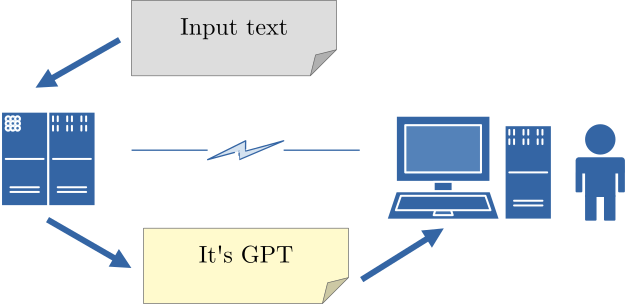
\includegraphics[width=0.7\linewidth]{images/Application/diagramma}
	\caption{Communication through RESTful API}
	\label{fig:diagramma}
\end{figure}

\section{Backend}

\paragraph{Technologies}
We used the following technologies:

\begin{itemize}
	\item \textbf{Flask} to create our backend as it provides an « ideal framework to build RESTful web services due to its lightweight nature » \cite{grinberg2018flask}.
	
	\item \textbf{Transformers}, a \textit{Hugginface}'s Python library « with the
	goal of opening up these advances [in higher-capacity model] to the
	wider machine learning community. The library consists of carefully engineered state-of-the art Transformer architectures under a
	unified API » \cite{wolf2020huggingfaces}.
	
	\item Optionally, \textbf{OpenAI's APIs} if GPT-3 is used as language model.
\end{itemize}

\subsection{Transformers}

\paragraph{Metric}
The function \texttt{evaluate\_texts} performs the operations described in Chapter \ref{chapter:meth}

\lstinputlisting[firstline=104,lastline=132,language=Python]
{../src/main.py}

\paragraph{Models}
To avoid using OpenAI's APIs, since they're metered \cite{openaiprice}, we've decided to use local models, such models are loaded through the Transformers library:

\lstinputlisting[firstline=20,lastline=24,language=Python]
{../src/main.py}

\paragraph{Perturbations}
Text's perturbation are generated as follows:

\lstinputlisting[firstline=25,lastline=62,language=Python]
{../src/main.py}

Basically we replace groups of tokens with a special token \texttt{<extra\_id\_$i$>}, which is then replaced by T5 with something it thinks fits well, basically rephrasing the text.

\subsection{RESTful API}

\paragraph{}
Our application has only one REST endpoint, \texttt{/evaluate}, such endpoint exposes the functionality \texttt{evaluate\_texts} to clients

\lstinputlisting[firstline=11,lastline=16,language=Python]
{../src/backend.py}

of course a big organization may decide to offload such computationally heavy task to the \textit{Cloud} and rely on OpenAI's metered services and their better-performing GPT models. Such approach would promote the system to a 3-tier system.

\section{Frontend}

\subsection{RESTful requests}

\lstinputlisting[firstline=10,lastline=32,language=Python]
{../src/app.py}

\subsection{GUI Features}

\paragraph{Folder Selection} One of the key features of our application is the ability to effortlessly select the 
target folder for document scanning and analysis. This ensures that users can easily pinpoint the location of the 
documents they want to process.

\paragraph{Document Preview} In the second section of the application, users are presented with a comprehensive 
view of the selected document. Here, they can examine the extracted text and view the results of the detection process.

\paragraph{Efficiency and Accuracy} Our application employs state-of-the-art algorithms to detect gpt-written 
text within documents. This ensures both efficiency and accuracy in identifying and processing relevant content.

\paragraph{Batch Processing} The real strength of our application lies in its batch processing capabilities. 
Users can queue up multiple documents within a selected folder, allowing for simultaneous scanning and analysis. 
This significantly reduces the time and effort required for handling a large number of documents.

\paragraph{User-Friendly Interface} With a focus on usability, our application boasts an intuitive interface. 
Even those with limited technical expertise can navigate through the process with ease, thanks to its simple and 
straightforward design.

\paragraph{Visual Aid} To provide a clearer picture of the application, we've included an image below that showcases 
its layout and features.

\begin{figure}
	\centering
	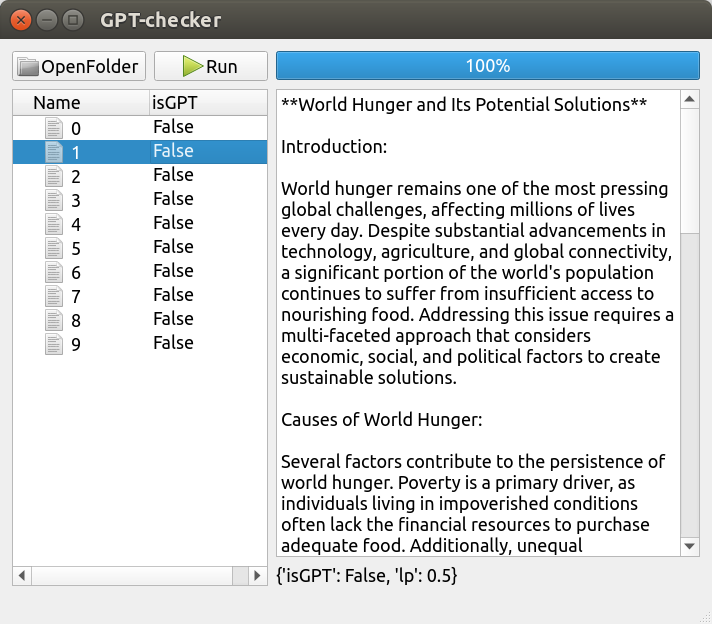
\includegraphics[width=0.9\linewidth]{images/Application/screen}
	\caption{Application's main window}
	\label{fig:screen}
\end{figure}

\paragraph{}
In conclusion, our innovative document scanning application powered by Python and Qt5 offers organizations a 
convenient and efficient solution for identifying and processing gpt-generated texts. Its user-friendly 
interface and batch processing capabilities make it an indispensable tool for enhancing productivity and accuracy 
in document management tasks.

\section{Source Code}
\paragraph{}
The implementation can be found on our git repository hosted on Github: \url{https://github.com/scarburato/gpt-tester}.